\documentclass[12pt]{article}
\usepackage{geometry}                % See geometry.pdf to learn the layout options. There are lots.
\geometry{letterpaper}                   % ... or a4paper or a5paper or ... 
%\geometry{landscape}                % Activate for for rotated page geometry
\usepackage[parfill]{parskip}    % Activate to begin paragraphs with an empty line rather than an indent
\usepackage{daves,fancyhdr,natbib,graphicx,dcolumn,amsmath,lastpage,url}
\usepackage{amsmath,amssymb,epstopdf,longtable}
\usepackage[final]{pdfpages}
\DeclareGraphicsRule{.tif}{png}{.png}{`convert #1 `dirname #1`/`basename #1 .tif`.png}
\pagestyle{fancy}
\lhead{CE 3354 -- Engineering Hydrology}
\rhead{FALL 2024}
\lfoot{ES1}
\cfoot{}
\rfoot{Page \thepage\ of \pageref{LastPage}}
\renewcommand\headrulewidth{0pt}



\begin{document}
\begin{center}
{\textbf{{ CE 3354 Engineering Hydrology} \\ {Exercise Set 2}}}
\end{center}

\section*{\small{Exercises}}
Figure \ref{fig:Texas-Training-Watershed-RFS} is a map of Harden Branch Creek area in Concho County, Texas. 
The \textbf{Assessment Point} on the map, conicides with the red circle below on Figure \ref{fig:hardinbranch-RFS}, which is centered on the bridge on US 87 just west of Eden Texas.\footnote{This watershed is the subject of the semester design project, PR-1.}

\begin{figure}[h!] %  figure placement: here, top, bottom, or page
   \centering
   \includegraphics[width=6in]{Texas-Training-Watershed-RFS.png} 
   \caption{Texas Training Watershed Map (annotated)}
   \label{fig:Texas-Training-Watershed-RFS}
\end{figure}

\begin{figure}[h!] %  figure placement: here, top, bottom, or page
   \centering
   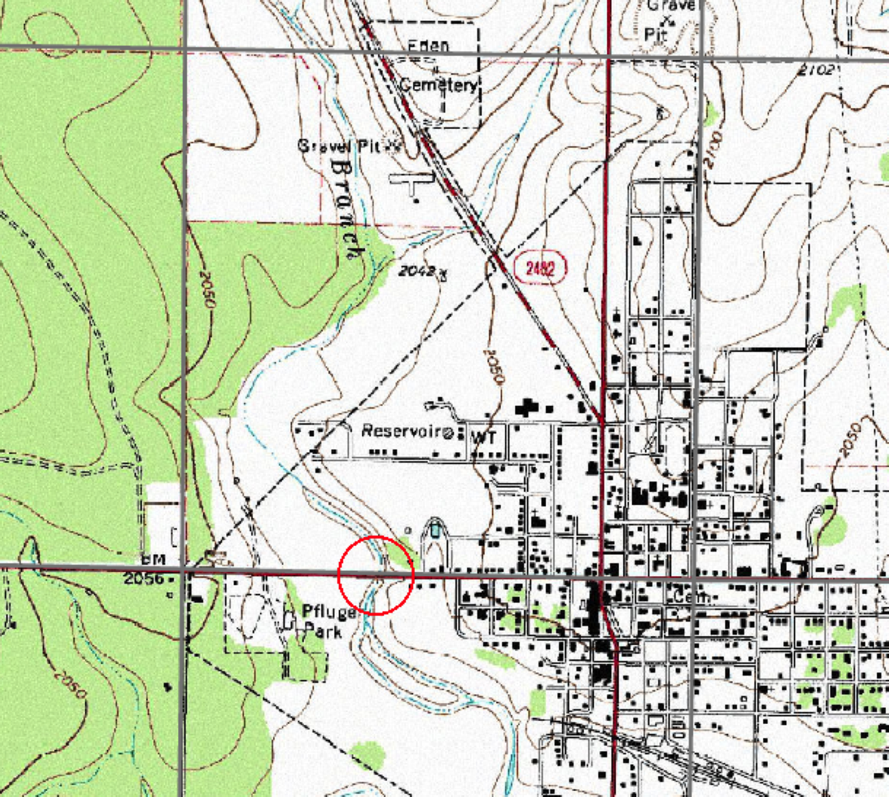
\includegraphics[width=6in]{hardinbranch-RFS.png} 
   \caption{Close-up of map West of Eden, Texas}
   \label{fig:hardinbranch-RFS}
\end{figure}

\begin{enumerate}
\item Using a GIS (i.e. QGIS) load an OpenStreetMap layer and locate the ``Assessment Point'' in the GIS.  Use the coordinate capture plug-in to capture the DD.DDD (decimal degrees) coordinates of the bridge.  Screen capture the GIS to demonstrate the determination of the coordinates.\footnote{The DD.DDD coordinates are mostly for this assignment only; A typical coordinate capture will report the coordinates as an ordered pair of degrees East (negative if West of the prime meridian,which Texas is) and degrees North (negative if south of the Equator).  Answers of (-100.00--ish, 30.00-- ish) are about right for this bridge. (precise values are for you to determine)}

\item Draw the boundary of the entire watershed area (i.e delineate the watershed)\footnote{You can use GIS tools such as System for Automated Geoscientific Analyses (SAGA) \url{https://saga-gis.sourceforge.io/en/index.html} or simply generate a map with contours, and by-hand delineate the watershed.  Use the Shuttle Radar Topography Mission (SRTM) \url{https://pubs.usgs.gov/publication/fs07103} as your source of elevation data.  QGIS has plug-in for both items; these are the same as demonstrated in class.} that drains to the red circle in Figure \ref{fig:hardinbranch-RFS}. Be sure to include the area of the two regulating structures (the earth berms/dams with riser pipe outlets) which also contribute to the outlet.

\item Determine the drainage area of the watershed in square miles.

\item Find the coordinates of the two outlet risers for the two SCS impoundments in the area; GoogleEarth might be helpful; a proper USGS Topographic map would also be helpful.  You will need these coordinates for future homework/project.

\item Determine the channel lengths from the watershed boundary to the SCS impoundments outlets.  

\item Determine the channel lengths from the SCS impoundment outlets to the junction where the two separate streams combine into the single stream (Hardin Branch).

\item Determine the channel length from the junction to the Bridge/culvert on US 87.

\item Determine elevation profiles along the two longest paths.


\end{enumerate}

Save the GIS project so you can use the tool(s) for additional terrain analysis.  If you do the exercise by-hand, save your original work; you will need it later on.

\end{document}  